\chapterauthor{Tim Warburton}

\epigraph{Debugging is twice as hard as writing the code in the first place. Therefore, if you write the code as cleverly as possible, you are, by definition, not smart enough to debug it}{Brian W. Kernighan}

\minitoc

In this lecture we discuss the following topics related to C programming:

\begin{itemize}
    \item Control flow:
        \item Conditional if statements.
        \item For loops.
        \item While loops.
    \item Functions.
    \item Function arguments passed by copy.
    \item Function scope.
    \item C structures (structs).
    \item \#include
    \item Math functions
\end{itemize}

\section{C control flow}

The system executes your program in a systematic fashion. It steps line by line through the list of statements. We can use the \texttt{if}, \texttt{for}, and \texttt{while} programming constructions to construct a program whose sequence of instructions depends on data (i.e. variables). In the following we discuss the role of each of these three flow control constructions.

\subsection{C conditional \texttt{if/else} statements}

Consider the following code and see if you can figure out the values of \texttt{a} and \texttt{b} at the end.
\begin{minted}{c}
  int a = 3;
  int b = 1;
  if(a==4){ /* a==4 evaluates to 1 if true and 0 if false */
    b = 2;
  }else{
    a = 2;
  }
\end{minted}
A moment's thought will reveal that initially \texttt{a=3} and \texttt{b=1} and then the expression \texttt{a==4} is evaluated. The double equals operator returns 1 if both arguments are the same or 0 otherwise. Since here \texttt{a} is set to 3 then it will evaluate to 0. That expressions is an \texttt{if/else} construct and since the argument of \texttt{if} evaluates to 0 the system will step into the \texttt{else} part of the expression, sometimes called taking the \texttt{else} branch. Inside the \texttt{else} branch the value of \texttt{a} will be set to 2. 

Thus at the end of this code snippet \texttt{a=2} and \texttt{b=1}. The value of \texttt{b} was never changed after initialization.

Here are some \texttt{if/else} expressions. See if you can figure out what the state of the variables are after execution. Look up the meaning of the following logical operators if you are unfamiliar with them:

{\bf Q1}:

\begin{minted}{c}
  int a = 3;
  int b = 1;
  if(a==3){ 
    b = 2;
  }else if(b==2){
    a = 2;
  }
\end{minted}

{\bf Q2}:

\begin{minted}{c}
  int a = 3;
  int b = 1;
  if(a!=3){ 
    b = 2;
  }else{
    a = 2;
  }
\end{minted}

{\bf Q3}:

\begin{minted}{c}
  int a = 3;
  int b = 1;
  if(a-3){ 
    b = 4;
  }else{
    a = 7;
  }
\end{minted}

{\bf Q4}:

\begin{minted}{c}
  int a = 3;
  int b = 1;
  if(b/a){ 
    b = 4;
  }else{
    a = 9;
  }
\end{minted}

{\bf Q5}:

\begin{minted}{c}
  int a = 3;
  int b = 1;
  if(!(b/a)){ 
    b = 4;
  }else{
    a = 9;
  }
\end{minted}

{\bf Q6}:

\begin{minted}{c}
  int a = 3;
  int b = 1;
  if((a==3) && (b!=2)){ 
    b = 4;
  }else{
    a = 9;
  }
\end{minted}

{\bf Q7}:

\begin{minted}{c}
  int a = 3;
  int b = 0;
  if((a==3) || (b==1)){ 
    b = 4;
  }else{
    a = 9;
  }
\end{minted}

Answers are in this footnote\footnote{Q1: \texttt{a=3,b=2}. Q2: \texttt{a=2, b=1} [\texttt{!=} is $\neq$]. Q3: \texttt{a=7, b=1} [ \texttt{a-3} evaluates to zero]. Q4: \texttt{a=9, b=1} [\texttt{b/a} evaluates to zero in integer arithmetic]. Q5: \texttt{a=3,b=4} [\texttt{!(b/a)=!(0)} and \texttt{!} is the NOT operator]. Q6: \texttt{a=3, b=4} [\texttt{\&\&} is the AND operator]. Q7: \texttt{a=3, b=4} [ \texttt(a==3) evaluates to 1, \texttt{b==3} evaluates to 0, and the OR operator \texttt{||} evaluates to 1 since one or more of its arguements are true}

\newpage
\subsection{C \texttt{for} loops}

The \texttt{for} loop is a supremely useful flow code construction that is incorporated into numerous programming languages (\href{https://en.wikipedia.org/wiki/For_loop#1972:_C/C++}{wiki on for loops}). 

Borrowing the wiki terminology a standard for loop in C has the following construction:
\begin{minted}{c}
for ([INITIALIZATION]; [CONDITION]; [INCREMENT]){
  [LOOP BODY]
}
\end{minted}

\begin{multicols}{2}[\columnsep2em] 

The C \texttt{for} loop executes as follows: 
\begin{enumerate}
    \item Evaluate INITIALIZATION expression.
    \item Evaluate CONDITION expression. 
    \item If the CONDITION expression evaluates to false then the \texttt{for} loop is completed. 
    \item Otherwise the LOOP BODY is executed then the INCREMENT step and the CONDITIONAL expression evaluated. 
    \item If the CONDITIONAL expression evaluates to false then the \texttt{for} loop is completed.
    \item This sequence of LOOP BODY + INCREMENT + CONDITIONAL check is repeated until the CONDITIONAL expression evaluates to false.  
\end{enumerate}

In the figure on the right we show a decision flow chart for the C for loop. In the following we give some example \texttt{for} loops in action.
\columnbreak

\begin{center}
    \fbox{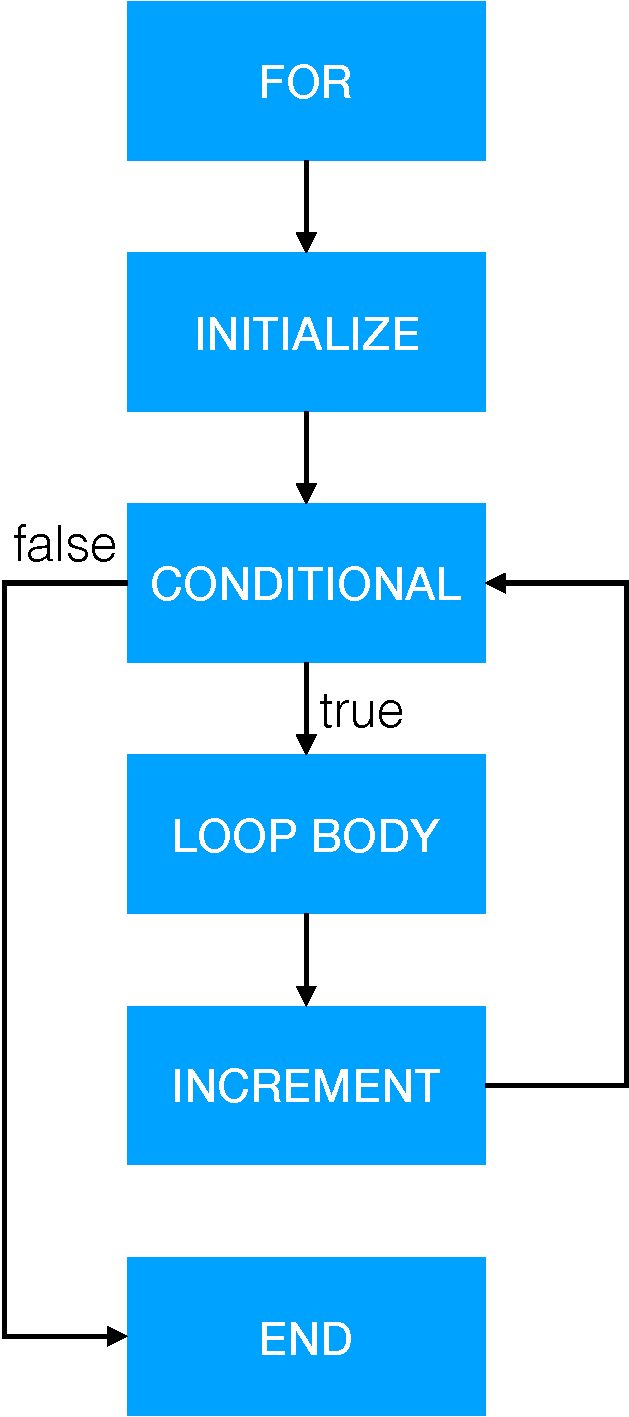
\includegraphics[width=0.3\textwidth]{figures/L07/CforLoopLogic.pdf}}
   \end{center}
\end{multicols}

{\bf For loop example \#1}: we can add up the first ten numbers with
\begin{minted}{c}
  int result = 0;
  int n;
  
  for(n=1;n<=10;n=n+1){
    result = result + n;
  }
\end{minted}

Here: the INITIALIZATION code is set \texttt{n=1}, the CONDITION evaluates the logical expression \texttt{n<=10} (i.e. $n\leq 10$), the INCREMENT code is \texttt{n=n+1} (i.e. increase \texttt{n} by 1), and the LOOP BODY is \texttt{result = result +n;} which adds $n$ to an accumulator variable called \texttt{result}.

{\bf For loop example \#2}: we can add up the even numbers up to and including ten with
\begin{minted}{c}
  int result = 0;
  int n;
  
  for(n=1;n<=10;n=n+1){
    if((n%2)==0){ /* is the number even, here % is mod op */
      result = result + n;
    }
  }
\end{minted}
But this takes 10 iterations to add up 5 numbers so we could do something a little smarter by adjusting the increment step
\begin{minted}{c}
  int result = 0;
  int n;
  
  for(n=2;n<=10;n=n+2){
    result = result + n;
  }
\end{minted}
Notice how the INITIALIZATION and INCREMENT CHANGED. Why did we change the INITIALIZATION code ?

There is no hard and fast written rule that says a \texttt{for} loop has to look like the above code. For instance the INITIALIZATION and INCREMENT expressions could be empty with the INITIALIZATION of variables performed before the loop and the INCREMENT performed inside the LOOP BODY. However, this might make it more difficult to parse the intent of the \texttt{for} loop when someone else tries to read the code. Thus many \texttt{for} loops follow the convention of including explicit INITIALIZATION and INCREMENT steps in the triad of arguments provided to the \texttt{for} loop.

\section{C Functions}

A C program is mostly just a collection of functions. In fact we have already seen the pivotal role of the \texttt{main} function. It is primary amongst all C functions as every C program must have a \texttt{main} function. The name is a giveaway too.

One style of programming is to put all C statements inside the \texttt{main} function and let the compiler sort it out. Pity any programmer who has to read such a code and figure out what it does. Programs tend to grow over time. Imagine a single function with 1000s of lines of code. A monolithic code like this is a nightmare to maintain and super difficult for multiple programmers to collaborate on.

A much more productive and common style of C programming is to divide a program into a set of functions. This raises a good question: when should I make a new function ? Advice on this varies, but one rule of thumb is if there is a sequence of operations that gets repeated several times then adding a function might be a good plan.

{\bf Example}: consider a simple 2-vector given by
\[
v = \left( \begin{array}{c}
v_0\\ v_1\end{array} \right).
\]
where $v$ is fully described by two real values $v_0$ and $v_1$.

In practice we will have many of these vectors on hand, for example recording the position of gravitating point particles in 2-space. There are several operations that will be required frequently, for instance in computing the Euclidean distance between two particles located at $v$ and $w$ given by
\[
| v - w | = \sqrt{(v_0-w_0)^2 + (v_1-w_1)^2}.
\]

To create a clean implementation of this we will break it into two parts: computing the difference between two 2-vectors,  computing the norm of a 2-vector.

{\bf Part 1}: Later we will turn this into a function too, but let's get started by initializing two 2-vectors and computing their difference

\begin{minted}{c}
float v0 =  1.0; // v = (1,2)
float v1 =  2.0;
float w0 =  2.0; // w = (2,-1)
float w1 = -1.0; 
float u0 = v0 - w0; // u = v - w
float u1 = v1 - w1;
\end{minted}

Notice how it is going to get super tedious if we have to keep doing this any time we want to subtract two vectors.

{\bf Part 2}: The norm operator denoted by $|.|$ is  a function that maps from 2-space ($\mathbb{R}^2$ in math notation) to the non-negative reals ($\mathbb{R}_{\geq0}$). 

To implement this in a simple way

\begin{minted}{c}
#include <stdio.h>
#include <math.h>

float vecNorm(float u0, float u1){
  float normu = sqrt(u0*u0+u1*u1);
  return normu;
}

int main(int argc, char **argv){

  float v0 =  1.0; // v = (1,2)                                                 
  float v1 =  2.0;
  float w0 =  2.0; // w = (2,-1)                                                
  float w1 = -1.0;
  float u0 = v0 - w0; // u = v - w                                              
  float u1 = v1 - w1;

  float normu = vecNorm(u0, u1);
  printf("|u| = |v-w| = %f\n", normu);

  return 0;
}
\end{minted}
In this example we only used \texttt{vecNorm} once, to compute $|v-w|$, so that is not a great win. But we could also use it to compute $|v|$ and $|w|$ with just one line of code each like this

\begin{minted}{c}
#include <stdio.h>
#include <math.h>

float vecNorm(float u0, float u1){
  float normu = sqrt(u0*u0+u1*u1);
  return normu;
}

int main(int argc, char **argv){

  float v0 =  1.0; // v = (1,2)                                                 
  float v1 =  2.0;
  float w0 =  2.0; // w = (2,-1)                                                
  float w1 = -1.0;
  float u0 = v0 - w0; // u = v - w                                              
  float u1 = v1 - w1;

  float normu = vecNorm(u0, u1);
  float normv = vecNorm(v0, v1);
  float normw = vecNorm(w0, w1);
  printf("|u|=%f, |v|=%f, |w|=%f\n", 
     normu, normv, normw);

  return 0;
}
\end{minted}
Capturing a ubiquitous function like the above norm example is definitely a good reason to make a new function.

There are a few caveats here. For instance the \texttt{vecNorm} function is only visible to code that comes after it in the file, i.e. I can only call the function from below the definition. When we have created a lot of functions it might become impossible to satisfy this constraint amongst the functions.

\subsection{Example: sine function}

The C math library contains a wide range of trig and other commonly used functions. If you have used sine or cosine functions in code have you pondered what happens inside the function.

\subsection{Extending where a function can be called from} 
As just mentioned a function is only visible to code that comes after it in a source file. This becomes very restrictive. Fortunately C offers a remedy. The idea is to create a so-called ``prototype'' that describes what the input and output signature of a function is. This can be put at the top of a source file, and the function can be defined elsewhere in the file or in fact in a separate file.

Here is an example that allows us to move the \texttt{vecNorm} function below the place it is called by predefining the function signature with a prototype at the start of the file.

\begin{minted}{c}
#include <stdio.h>
#include <math.h>

/* prototype for vecNorm describing its function signature */
float vecNorm(float , float );

int main(int argc, char **argv){

  float v0 =  1.0; // v = (1,2)                                                 
  float v1 =  2.0;
  float w0 =  2.0; // w = (2,-1)                                                
  float w1 = -1.0;
  float u0 = v0 - w0; // u = v - w                                              
  float u1 = v1 - w1;

  float normu = vecNorm(u0, u1);
  float normv = vecNorm(v0, v1);
  float normw = vecNorm(w0, w1);
  printf("|u|=%f, |v|=%f, |w|=%f\n", 
     normu, normv, normw);

  return 0;
}

/* actual definition of function */
float vecNorm(float u0, float u1);
{
  float normu = sqrt(u0*u0+u1*u1);
  return normu;
}
\end{minted}

With this approach it is sufficient to list the prototypes of a set of functions, and that extends the scope of their usage without imposing an ordering on them in the source file that satisfies their inter-dependency. 

We will revisit the use of prototypes later when we dive into header files and multiple source file projects.

\subsection{Scope of function variables}

There are some important details we glossed over in the introduction of a function. In this \texttt{vecNorm} example function we need to dissect what happens when it gets called.

\begin{minted}{c}
float vecNorm(float u0, float u1);
{
  float normu = sqrt(u0*u0+u1*u1);
  return normu;
}
\end{minted}
The most potentially confusing aspect is that when it gets called from \texttt{main} with
\mint{c}|float normu = vecNorm(u0, u1);| 

the values of \texttt{u0} and \texttt{u1} are copied into new variables. On entry to the \texttt{vecNorm} function two new variables are created, and the values of the variables from the \texttt{main} function are copied into these new variables. This mechanism for passing variable values into the function is referred to as pass-by-copy. 

The argument pass-by-copy mechanism has some significant repercussions. We will illustrate these with some example codes.

In the following code the function  \texttt{foo} is called from \texttt{main}. Function \texttt{foo} accepts one argument variable, and it changes the value of that variable. Then when execution passes back to \texttt{main} there is a print statement. Without looking at the explanations below, what do you think will be printed ?

\begin{minted}{c}
void foo(int a){
  a = 3;
}

int main(int argc, char **argv){
  
  int b = 1;
  
  foo(b);
  printf("b=%d\n", b);

  return 0;
}
\end{minted}

If you thought to yourself that the output should be $b=1$ then you are correct. When \texttt{b} was passed into the function \texttt{foo} a new \texttt{int} variable was created called \texttt{a} that was purely local to the scope of the \texttt{foo} function. That function change the value of the local variable to 3, but since it was changing a copy when the function exited there was no modification to the \texttt{a} variable that resided purely in the \texttt{main} function scope.

If we had wanted to pass a value back from \texttt{foo} and assign that value to the \texttt{main} variable \texttt{b} then we could have done the following 

\begin{minted}{c}
int foo(int a){
  a = 3;
  return a;
}

int main(int argc, char **argv){
  
  int b = 1;
  
  b = foo(b);
  printf("b=%d\n", b);

  return 0;
}
\end{minted}
and we would see the printout \texttt{b=3}. The argument value was passed into \texttt{foo} as a copy, and the return value was passed by copying from \texttt{a} to \texttt{b}.

A reasonable question: is copying the only way that data can be accessed or modified by a function ? Can a function output more than one variable ? 

Fortunately we can circumvent some of these restrictions. In the following we will discuss two ways of increasing the input and output options for a function.

\newpage
\section{C structures (structs)}

In the previous section we started to see some limitations caused because C uses a pass-by-copy mechanism for function arguments and return values. Since there is only one output variable it might appear that a function can only return one value.

One way to increase the amount of data that can be passed to and from a function is to bundle multiple variables into a composite variable. In C we can define a new variable type that collects multiple variables of varying type into a so-called ``struct''.

In the above example we used two separate \texttt{float} variables to encode the two components of a 2-vector. We could have alternatively created a new variable type called say \texttt{vec2} that contains the two component variables. As follows

\begin{minted}{c}
typedef struct {
   float x;
   float y;
} vec2;
\end{minted}

We can now use this new variable type anywhere below this definition in the source file. In the following example we repeat the example code from above but this time using the \texttt{vec2} variable type.

\begin{minted}{c}
typedef struct {
   float x, y;
} vec2;

/* prototypes */
float vecNorm(vec2);
vec2  vecSubtract(vec2, vec2);

int main(int argc, char **argv){

  vec2 u, v, w;
  v.x = 1.0; /* v = (1,2) */
  v.y = 2.0;
  w.x = 2.0; /* w = (2,-1) */
  w.y = -1.0;
  
  u = vecSubtract(v,w); /* u = v-w */
 
  float normu = vecNorm(u);
  float normv = vecNorm(v);
  float normw = vecNorm(w);
  printf("|u|=%f, |v|=%f, |w|=%f\n", normu, normv, normw);

  return 0;
}

/* actual definition of functions */
float vecNorm(vec2 u);
{
  float normu = sqrt(u.x*u.x+u.y*u.y);
  return normu;
}
float vecSubtract(vec2 v, vec2 w);
{
  vec2 u;
  u.x = v.x-w.x;
  u.y = v.y-w.y;
  return u;
}
\end{minted}

The \texttt{emacs} source code highlighter does not know how to color code the \texttt{vec2} variable type. But after the definition of the \texttt{vec2} variable type the compiler certainly knows how to treat every instance of a \texttt{vec2} variable. 

We sneakily introduced one more piece of technology. The dot operator allows us to get to the member variables of the struct variable. For example

\mint{c}|v.x = 1.0;| 

assigns the value one to the \texttt{x} member variable of the \texttt{v} variable. 

Finally, we can clean up the code a little more by observing that we might want to create several \texttt{vec2} variables. Our guiding light for when to create a new function is do so if we will repeatedly perform an action. So we tidy up the code by creating a \texttt{vecCreate} function that will take an argument each for  \texttt{x} and \texttt{y} and return a populated instance of a \texttt{vec2} struct as follows.

\begin{minted}{c}
typedef struct {
   float x, y;
} vec2;

/* prototypes */
float vecNorm(vec2);
vec2  vecCreate(float, float);
vec2  vecSubtract(vec2, vec2);

int main(int argc, char **argv){

  vec2 v = vecCreate(1.0, 2.0);
  vec2 w = vecCreate(2.0, -1.0);
  vec2 u = vecSubtract(v,w); /* u = v-w */
 
  float normu = vecNorm(u);
  float normv = vecNorm(v);
  float normw = vecNorm(w);
  printf("|u|=%f, |v|=%f, |w|=%f\n", normu, normv, normw);

  return 0;
}
\end{minted}
We have created a relatively transparent piece of code and incidentally are starting on the process of creating a C struct that encapsulates data associated with a 2-vector and a library of C functions that implement certain operations that we might wish to perform with a 2-vector. Can you think of other operations that might be useful to add to this growing library ?

During our encapsulation of data and operations we have started to hide the struct member variables away from the \texttt{main} function level code. Notice how only the library of \texttt{vec2} functions actually access member variables. 
\begin{minted}{c}
/* actual definition of functions */
vec2 vecCreate(float x, float y){
  vec2 u;
  u.x = x;
  u.y = y;
  return u;
}

float vecNorm(vec2 u){
  float normu = sqrt(u.x*u.x+u.y*u.y);
  return normu;
}

vec2 vecSubtract(vec2 v, vec2 w){
  vec2 u;
  u.x = v.x-w.x;
  u.y = v.y-w.y;
  return u;
}
\end{minted}

\section{C header files}

The list of functions that manipulate the \texttt{vec2} struct is growing. If a struct and associated set of interface functions  is going to be used in multiple places in a code it makes sense to gather the definition of the struct and the functions into a so called ``header'' file (sometimes also called an ``include'' file). The \texttt{stdio.h} and \texttt{stdlib.h} standard C header files are examples of header files provided with the C compiler and follow the convention of having a \texttt{.h} suffix.

The syntax in header files is standard C. A typical header file may include definitions of struct types and the ''prototypes'' for the related functions that use the structs. For this usage of the word a prototype for a function includes the:

\begin{enumerate}
    \item The type of the returned value.
    \item The name of the function.
    \item The type of each of the arguments.
    \item A terminating semi-colon.
    \item An optional comment for each function prototype.
\end{enumerate}

In the following header called \texttt{vec2.h} we include a definition of the \texttt{vec2} struct and API function prototypes with some optional comments about their purpose.

\begin{minted}{c}
/* vec2.h */

/* make sure that this header has not been defined already */
#ifndef __VEC2
#define __VEC2 1

typedef struct {
   float x, y;
} vec2;

/* vec2 constructor */
vec2 vecCreate(float , float );

/* Euclidean norm of vec2 */
float vecNorm(vec2 );

/* Return v-w */
vec2 vecSubtract(vec2 v, vec2 w);

#endif
\end{minted}

{\bf Note \#1}: we wrap the contents of the \texttt{vec2.h} header file with a guard compiler directive to make sure that the contents of the header are not included twice in the same source file.

{\bf Note \#2}: we can include this header file at the top of a source file with 

\begin{minted}{c}
#include "vec2.h"
\end{minted}

But we will still have to provide the actual implementations of these \texttt{vec2} API functions at some point in the file unless we place those function implementations in a separate file and create a multiple C source file project.

\section{C multiple file projects}

In the last section we saw how we can create a header file that describes a struct and the form of the function prototypes involving that struct. In this section we show how to split the API functions into \texttt{vec2.c}, the \texttt{main} function into \texttt{vec2Main.c}.

C allows us to separate functions into separate source code files. Thus we can separate the above code into a \texttt{vec2Main.c} file

\begin{minted}{c}
#include <stdio.h>
#include "vec2.h"

int main(int argc, char **argv){

  vec2 v = vecCreate(1.0, 2.0);
  vec2 w = vecCreate(2.0, -1.0);
  vec2 u = vecSubtract(v,w); /* u = v-w */
 
  float normu = vecNorm(u);
  float normv = vecNorm(v);
  float normw = vecNorm(w);
  printf("|u|=%f, |v|=%f, |w|=%f\n", normu, normv, normw);

  return 0;
}
\end{minted}

and a separate \texttt{vec2.c} file

\begin{minted}{c}
#include <stdio.h>
#include "vec2.h"

vec2 vecCreate(float x, float y){
  vec2 u;
  u.x = x;
  u.y = y;
  return u;
}

float vecNorm(vec2 u);
{
  float normu = sqrt(u.x*u.x+u.y*u.y);
  return normu;
}

vec2 vecSubtract(vec2 v, vec2 w);
{
  vec2 u;
  u.x = v.x-w.x;
  u.y = v.y-w.y;
  return u;
}
\end{minted}

The observant reader will notice that we used the convention \texttt{\#include <stdio.h>} when including the standard IO header and \texttt{\#include "vec2.h"} for our own header file. The former notation with \texttt{<...>} is typically reserved when include a standard system header file and \texttt{"..."} when including user supplied header files.

Thus we now have a three file project:

\begin{itemize}
    \item[] \texttt{vec2.h}: contains the \texttt{vec2} struct type definition and prototypes for the API functions.
    
    \item[] \texttt{vec2Main.c}: contains the implementation of the \texttt{main} function. {\bf Note}: it includes the \texttt{vec2.h} header file.
    
    \item[] \texttt{vec2.c}: contains the implementations for the \texttt{vec2} struct API functions. {\bf Note}: it also includes the \texttt{vec2.h} header file.
\end{itemize}

The simplest way to compile this three file project is to include all the \texttt{.c} files in the compiler arguments.

\myvbox[mytermbg]{gcc -I./ -o vec2Main vec2Main.c vec2.c -lm}

There are two new components to this compiler command. We added \texttt{-I./} to direct the compiler to look for header files in the present working directory. We also added the \texttt{-lm} option at the end of the compile line to force the compiler to also combine the standard C math library when building the \texttt{main} executable (important since we use the \texttt{sqrt} function that is part of the math library).

